%% SECTION HEADER /////////////////////////////////////////////////////////////////////////////////////
\section{Temperature effect on the \acs{gw} propagation}
\label{sec:temp}
 
\ac{gw} propagate from actuator to sensor in very short time (in miliseconds) in comparison to slow changes in ambient temperature (in seconds).
Therefore, \ac{gw} propagation can be modelled for the stationary temperature field.
It is assumed that the temperature field can be obtained from temperature sensors at the moment of \ac{gw} excitation.
A uniform temperature field was assumed in the model for simplicity.

In order to carry out the temperature-dependent \ac{sem} simulations, only changes in the elastic modulus of the \ac{hsc} components are considered.
The density changes are neglected.
The mechanical properties for the components of the analysed \ac{hsc} panel at the reference temperature \(T_r=20\)\unit{\degreeCelsius} are included in Tab. \ref{tab:properties}.
\begin{table}[H]
	\small
	\tabcolsep=0.5cm
	\centering
	\caption{\label{tab:properties}The mechanical properties of the materials at reference temperature of +20\unit{\degreeCelsius}.}
	\begin{tabular}{ccccc}\toprule
		\multirow{2}{*}{\textbf{Material}} & $\boldsymbol{E_{11}}$ & $\boldsymbol{E_{33}}$ & $\boldsymbol{\nu_{12}}$ & $\boldsymbol{\rho}$ \\ & \unit{\giga\pascal} & \unit{\giga\pascal} & -- & \unit[per-mode = symbol]{\kilogram\per\cubic\meter}\\
		\midrule
		Carbon & 275 & 27 & 0.2 & 1900\\
		Epoxy & 3.43 & 3.43 & 0.35 & 1250\\
		Aluminium & 69 & 69 & 0.33 & 2770\\
		Epoxy adhesive & 6 & 6 & 0.34 & 1200\\
		Cyanoacrylate glue & 3 & 3 & 0.34 & 1200\\	
		\ac{pzt} &  59 & 47 & 0.31 & 7850\\
		\bottomrule
	\end{tabular}
\end{table}
For the \ac{cfrp} skin, the modulus is calculated as per the methodology described in \cite{chamis1983simplified,salamone2009guided}.
The significant changes in mechanical properties under temperature occur mainly in the polymer matrix, while the variation in the carbon fibre properties has a negligible effect on wave propagation.
In this model \cite{salamone2009guided, hopkins2012extreme}, the reduction of Young’s modulus of the resin \(E_m\) with temperature variation is assumed as:
\begin{eqnarray}
	E_m(T)=F_m E_{m}(T_r),
	\label{eq:factor_temp}
\end{eqnarray}
\nomtypeR[E]{$E$}{Young's modulus}{-}{\unit{\giga\pascal}}%
\nomtypeR[T]{$T$}{Temperature}{-}{\unit{\degreeCelsius}}%
\nomtypeR[Tr]{$T_r$}{Reference temperature}{-}{\unit{\degreeCelsius}}%
where \(E_{m}(T_r)\) is the Young’s modulus of resin at the reference temperature and \(F_m\) is the temperature degradation factor as proposed in \cite{chamis1983simplified}:
\begin{eqnarray}
F_m=\sqrt{\frac{T_{g0}-T}{T_{g0}-20}},
\label{eq:em_temp}
\end{eqnarray}
\nomtypeD[Fm]{$F_m$}{Temperature degradation factor}{\(\sqrt{\frac{T_{g0}-T}{T_{g0}-T_r}}\)}{}%
\nomtypeR[Tg0]{$T_{g0}$}{Glass transition temperature}{}{\unit{\degreeCelsius}}%
where \(T_{g0}\) is the glass transition temperature.

Temperature-dependent properties of \ac{cfrp} skin are presented in Fig. \ref{fig:cfrpEG}.
\begin{figure}
	\begin{center}
		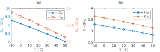
\includegraphics[width=0.95\textwidth]{Chapter_3/cfrpEG}
	\end{center}
	\caption{Temperature-dependent \textbf{(a)} Young's modulus (E\(_{11}\), E\(_{33}\)) and \textbf{(b)} shear modulus (G\(_{12}\), G\(_{23}\)) for the \acf{cfrp} skin}
	\label{fig:cfrpEG}
\end{figure}

Eq. (\ref{eq:em_temp}) is also applicable to determine the elastic modulus of the adhesive layer bonding of the core to the skins, while for aluminium, the linear temperature dependence given by Hopkins et al. \cite{hopkins2012extreme} as:
\begin{eqnarray}
	E_a(T)=E_a(T_{r})+\num{4e7}(20-T).
	\label{eq:aluminium_temp}
\end{eqnarray}

Temperature-dependent properties of isotropic materials determined according to the formulas and the fact shear and Young's modulus are in relation as \(E=2G(1+\nu)\), are presented in Fig. \ref{fig:isoEG}.
\begin{figure}
	\begin{center}
		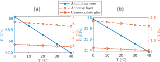
\includegraphics[width=0.95\textwidth]{Chapter_3/isoEG}
	\end{center}
	\caption{Temperature-dependent \textbf{(a)} Young's modulus (E) and \textbf{(b)} shear modulus (G) for isotropic materials used in the simulations.}
	\label{fig:isoEG}
\end{figure}

The Young's modulus and Poisson's ratio of the sensors are in the form proposed by Lanza et al. \cite{lanza2008temperature}:
\begin{eqnarray}
	\left(E_{11}\right)_{pzt}(T) & = & \left[\left(E_{11}\right)^{-1}_{pzt}(T_r) + \num{2.142857e-14}(20-T)\right]^{-1},\\
	\left(E_{33}\right)_{pzt}(T) & = & \left[\left(E_{33}\right)^{-1}_{pzt}(T_r) + \num{0.777142e-14}(20-T)\right]^{-1},\\
	\nu_{pzt}(T) & = & \nu_{pzt}(T_r) + \num{13e-3}(20-T).
	\label{eq:pzt_temp}
\end{eqnarray}
\nomtypeD[nu]{\( \nu \)}{Poisson's ratio}{-}

The piezo- and electromechanical properties are taken into account based on the
temperature characteristics provided by the manufacturer.
\begin{figure}
	\begin{center}
		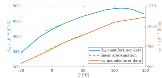
\includegraphics[width=0.95\textwidth]{Chapter_3/pzt_piezo_temp}
	\end{center}
	\caption{Temperature-dependent \textbf{(a)} Young's modulus (E\(_{11}\), E\(_{33}\)) and \textbf{(b)} shear modulus (G\(_{12}\), G\(_{23}\)) for the \acf{cfrp} skin}
	\label{fig:pzt_temp}
\end{figure}
The characteristics are approximated by the linear functions  in the analysed range (see Fig. \ref{fig:pzt_temp}) given in the form:
\begin{eqnarray}
	\textbf{d}(T) & = & \boldsymbol{d}(T_r) + \left[
	\begin{array}{cccccc}
		0 & 0 & 0 & 0 & 0 & 0\\
		0 & 0 & 0 & 0 & 0 & 0\\
		0.71 & 0.71 & -1.74 & 0 & 0 & 0
	\end{array}\right]\,(20-T) \times10^{-12},\\
	\boldsymbol{\epsilon}^S(T) & = & \boldsymbol{\epsilon}^S(T_r) - \left[
	\begin{array}{ccc}
		3.61 & 0 & 0\\
		0 & 3.61 & 0\\
		0 & 0 & 3.28
	\end{array}\right]\,(20-T) \times10^{-11},\\
	\textbf{e}(T) & = & \textbf{d}(T)\,\textbf{c}_{PZT}(T),
	\label{eq:piezo_temp}
\end{eqnarray}
\nomtypeG{\(\epsilon\)}{Electric permittivity}{-}{\unit[per-mode = symbol]
{\farad\per\metre}}%
\nomtypeR[d]{\(d\)}{Piezoelectric coupling coefficient}{-}{\unit[per-mode = symbol]
{\coulomb\per\newton}}%
\nomtypeR[e]{\(e\)}{Piezoelectric coupling coefficient}{-}{\unit[per-mode = symbol]
{\coulomb\per\square\metre}}%
were \(\boldsymbol{\epsilon}^S\) is the electric permittivity measured at zero strain, \(\boldsymbol{d}\) is the charge constant matrix, \(\boldsymbol{e}\) is the piezoelectric coupling coefficients matrix and \(\boldsymbol{c}_{PZT}\) is the elastic stiffness matrix.
The piezo constant matrices for reference temperature are provided by manufacturer as follows:
\begin{eqnarray}
	\textbf{d}(T_r) & = & \left[
	\begin{array}{cccccc}
	0 & 0 & 0 & 0 & 669 & 0\\
	0 & 0 & 0 & 669 & 0 & 0\\
	-208 & -208 & 443 & 0 & 0 & 0
	\end{array}\right] \times10^{-12}\ \unit[per-mode = symbol]{\coulomb\per\newton},\\
	\boldsymbol{\epsilon}^S(T_r) & = & \left[
	\begin{array}{ccc}
	802 & 0 & 0\\
	0 & 802 & 0\\
	0 & 0 & 729
\end{array}\right] \times10^{-11}\ \unit[per-mode = symbol]{\farad\per\meter},
\end{eqnarray}

The complete set of temperature-dependent coefficients for the \ac{pzt} are shown in Figs.~\ref{fig:pztEG}-\ref{fig:pztEEps}.

\begin{figure}
	\begin{center}
		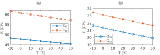
\includegraphics[width=0.95\textwidth]{Chapter_3/pztEG}
	\end{center}
	\caption{Temperature-dependent \textbf{(a)} Young's modulus (E\(_{11}\), E\(_{33}\)) and \textbf{(b)} shear modulus (G\(_{12}\), G\(_{23}\)) for the \acf{pzt}}
	\label{fig:pztEG}
\end{figure}
\begin{figure}
	\begin{center}
		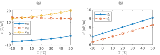
\includegraphics[width=0.95\textwidth]{Chapter_3/pztEEps}
	\end{center}
	\caption{Temperature-dependent \textbf{(a)} piezoelectric coupling coefficients (e\(_{31}\), e\(_{15}\), e\(_{33}\) and \textbf{(b)} electric permittivity (\(\boldsymbol{\epsilon}^S_{11}\), \(\boldsymbol{\epsilon}^S_{33}\)) for the \acf{pzt}}
	\label{fig:pztEEps}
\end{figure}
\nomtypeG[\(\rho\)]{\( \rho \)}{Mass density}{-}{\unit[per-mode = symbol]
	{\kilogram\per\cubic\metre}}